%% LyX 2.2.1 created this file.  For more info, see http://www.lyx.org/.
%t% Do not edit unless you really know what you are doing.
%\documentclass[english]{article}
%\usepackage[latin9]{inputenc}

%\usepackage{babel}
%begin{document}

\documentclass[english]{article}
\usepackage[T1]{fontenc}
\usepackage[latin9]{inputenc}
\usepackage[a4paper]{geometry}
\usepackage{amsmath}
\geometry{verbose,tmargin=2cm,bmargin=2cm,lmargin=2cm,rmargin=2cm}
\usepackage{graphicx}
%\usepackage[chapter]{algorithm}
\usepackage{algorithmic}
\usepackage{tabularx}
\usepackage{colortbl}
\usepackage{hhline}
\newcommand{\norm}[1]{\left\lVert#1\right\rVert}

\DeclareMathOperator*{\argmin}{\arg\!\min}
\DeclareMathOperator*{\argmax}{\arg\!\max}

\makeatletter

%%%%%%%%%%%%%%%%%%%%%%%%%%%%%% LyX specific LaTeX commands.
%% Because html converters don't know tabularnewline
\providecommand{\tabularnewline}{\\}

\makeatother

\usepackage{babel}
\begin{document}

\title{Machine Learning for Computer Vision (EE5177) \\ Programming Assignment 4 : Logistic Regression and SVMs \\ Problem \#3}

\author{Akshit Kumar \\ \emph{EE14B127}}

\date{17th April 2017}

\maketitle
\tableofcontents{}

\section{Introduction}

\subsection{Goal}
The goal of this question is to compare logistic regression and SVM by classifying a dataset with 4 classes ie multiclass classification. 

\subsection{Approach}
To do Logistic Regression, we make use of the \emph{glmnet} library and use it to train and test our logistic regression model.
To do SVM classification, we make use of the \emph{libsvm} library and use it to train and test our SVM classifier.
For training the model, a lot of work in hyperparameter tuning has gone, where we divide the training set into training set and cross validation set. Find the optimal value using the minimum cross validation set error and use those parameters for testing. We make use of n-fold cross-validation for determining the best parameters.

\subsection{Result Summary}
The RBF Kernel for SVM and logistic regression perform equally well giving an accuracy of \emph{70\%} and linear Kernel for SVM performs badly and is also slow.

\section{Logistic Regression}
\subsection{Approach}
Logistic regression is performed using \emph{glmnet}. \emph{glmnet} performs a log search for the kernel parameter $\lambda$ and the model returned contains all the values of $\lambda$ used. To find the best possible value of $\lambda$ we use n-fold cross validation. We use the value n = 10 to perform n-fold cross search. To do this we use the function \emph{cvglmnet} which performs n-fold cross validation on all the values of $\lambda$ given by glmnet to return the best value of $\lambda$.
\subsection{Result}
\begin{itemize}
	\item Accuracy = 70 \%
	\item $lambda_{min}$ = 0.0055
 	\item $lambda_{1se}$ = 0.0128
\end{itemize}


\begin{itemize}
	\item Cost Function : $L = \Sigma_{i=1}^{I} w_{i}log[\dfrac{1}{1 + \exp(-\phi^Tx_{i})}] + \Sigma_{i=1}^{I} (1-w_{i})log[\dfrac{\exp(-\phi^Tx_{i})}{1 + \exp(-\phi^Tx_{i})}]$ 
	\item Gradient : $\frac{\partial L}{\partial \phi} = -\Sigma_{i=1}^{I} (sig[a_{i}] - w_{i})x_{i}$
	\item Hessian : $\frac{\partial^{2} L}{\partial \phi^2} = -\Sigma_{i=1}^{I} sig[a_{i}](1 - sig[a_{i}])x_{i}x_{i}^T$
\end{itemize}
\subsection{Results}
The optimal values obtained on one trial of the experiment are :(Note : Since the points are sampled randomly, each time we get different optimal points as data changes)
\begin{itemize}
	\item Optimal $\phi$ : $\phi = \begin{bmatrix} 0.31 \\ 2.46 \end{bmatrix}$ 
	\item Gradient at Optimal $\phi$ : $\begin{bmatrix} -8.63e-05 \\ -0.00026 \end{bmatrix}$
	\item Hessian at Optimal $\phi$ : $\begin{bmatrix} 0.0898 & 0.0898 \\ 0.0898 & 0.0898 \end{bmatrix}$
\end{itemize}

\section{Issue with Linear Separability of Data}
When the data is linearly separable, there is an incentive for $\phi$ to get bigger and bigger, to \emph{emphasize} more and more the difference between the two classes. For example, if you double the size of $\phi$, then elements in class 1 get bigger log odds and elements in class 0 get smaller log odds. So from the prespective of minimizing the loss function, it is always better to make $\phi$ bigger and bigger. In this way, $\phi$ won't converge.
One way to deal with the issue is to add regularization to the cost function which penalizes the $\phi$ vector for becoming too large.

\section{Experiment Results}
\subsection{Confusion Matrix}
The confusion matrix obtained is as follows :
$$
\begin{tabularx}{.7\textwidth}{&gt;{\bfseries}c|c c c |}
 & Class 1 & Class 0 \\
\hhline{----}
Class 1 & 19 (tp) \cellcolor[gray]{.8}& 1 (fn)   \\
Class 0 & 0 (fp) & 20 (tn) \cellcolor[gray]{.8} \\
\hhline{~---}
\end{tabularx}
$$
\subsection{Required Plots}
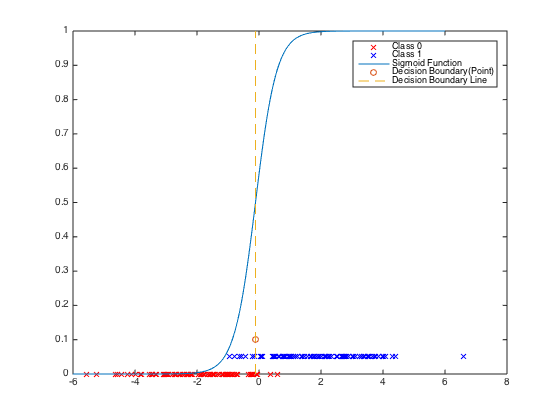
\includegraphics[scale=0.9]{../plot/plot}
\end{document}

